

\documentclass[a4paper, 10pt]{scrreprt}

%%%%%%%% Fonts and Encoding
\usepackage[ngerman]{babel}
\usepackage[utf8]{inputenc}
\usepackage[sc]{mathpazo}		%Palatino Font
\usepackage[svgnames]{xcolor}	%svgnames for RGB colors
\usepackage[T1]{fontenc}
\linespread{1.44}				%only with Palatino
\usepackage{microtype}
\DisableLigatures{encoding=T1,family=tt*}

%%%%%%%% Standard Packages
\usepackage{fancyhdr, graphicx, amsmath, amssymb, amsthm, bm, mathrsfs, paralist, shadethm, xspace}
%%%%%%%%
%\graphicspath{{./Bilder/}{./Bilder/Raman/}{./Bilder/Technik/}{./Bilder/Messungen/}{./Bilder/Auswertung/}{./Bilder/Titel/}{./Bilder/BaFeAs/}}
%%%%%%%%
\usepackage{subfig} % make it possible to include more than one captioned figure/table in a single float
\usepackage{multirow}
%%%%%%%% Hyperref Setup
\usepackage[pdftex, colorlinks=true,linkcolor=DarkBlue, urlcolor=black, citecolor=DarkGreen]{hyperref}
%%%%%%%
%\renewcommand{\thefigure}{\thesection.\arabic{figure}} 
%\renewcommand{\thetable}{\thesection.\arabic{table}} 

%%%%%%%% Andi...
\usepackage[inline]{enumitem}
\usepackage{geometry}
\geometry{bottom=1.5in}

\usepackage{nicefrac}

\usepackage{tikz}
\usetikzlibrary{arrows}
\usetikzlibrary{decorations.pathmorphing}
\usetikzlibrary{intersections}
\usetikzlibrary{calc}
\usetikzlibrary{patterns}
\usetikzlibrary{backgrounds}

\hypersetup{pdftitle={Titel}, pdfauthor={Ziegler, Maximilian}, pdfsubject={irgendwas}, pdfkeywords={Technische Universität München}, pageanchor=true}

%%%%%%%% Header and Footer (fancy)
\pagestyle{fancy}
\fancyhf{}
\renewcommand{\headrule}{{\color{gray} \hrule width\headwidth height\headrulewidth \vskip-\headrulewidth}}
\setlength{\headheight}{15pt}
%\fancyhead[R]{\color{gray}\slshape \nouppercase\rightmark}
\fancyhead[L]{\color{gray}\slshape \nouppercase\leftmark}
\fancyfoot[C]{\color{gray}\oldstylenums{\thepage}}

\fancypagestyle{plain} 
\fancyhf{}
\fancyfoot[C]{\color{gray}\oldstylenums{\thepage}}\renewcommand{\headrulewidth}{0pt} 

%%%%%%%% Newcommand 
\newcommand{\bfa}{BaFe\textsubscript{2}As\textsubscript{2}\xspace}
\newcommand{\bfca}{Ba(Fe\textsubscript{1-x}Co\textsubscript{x})\textsubscript{2}As\textsubscript{2}\xspace}
%%%%%%%%
%%%%%%%% Document Information
\author{Maximilian Ziegler}
\title{Titel}
\date{\today}

%%%%%%%% Main Document
\begin{document}

%%%%%%%% Title Page
\begin{titlepage}
%\setcounter{page}{0}
\clearpage \thispagestyle{empty} \setcounter{page}{0}
%\renewcommand{\arraystretch}{1}%     Felder der Tabellen wieder verkleinern

\begin{center}
\begin{figure}[h]
\centering

\end{figure}
\vspace{1.5cm}

%



%\end{center}
%
%\begin{figure}[H]
%\centering
{\centering
	{\huge 


		Fortgeschrittenenpraktikum							\\
		\vspace{2cm}
		
		{\bf	Mößbauereffekt	}										\\
		\vspace{1.5cm}
		
		Ausarbeitung												\\
		\vspace{1cm}
		
		Robin Häcker, Matrikel 03626146						\\
		\vspace{1cm}
		
		Philipp Klose, Matrikel 03631983						\\
		\vspace{1cm}
		
		Maximilian Ziegler, Matrikel 03638495						\\
		\vspace{1cm}
		
		22.10.2013												\\
		\vspace{1cm}
		
		Gruppe 136													\\
	}}
%\end{figure}
\end{center}
\end{titlepage}
%
\clearpage \thispagestyle{empty} \setcounter{page}{0}
\newpage \thispagestyle{empty}
\tableofcontents
\newpage
%%%%%%%%
\pagenumbering{arabic}

\chapter{Einleitung}
\label{cha:Einleitung}

	Bei Atomkernen in Festkörpern kann, wenn bestimmte Bedingungen erfüllt sind, rückstoßfreie, nicht thermisch verbreiterte Resonanzabsorptionen von Gammastrahlen beobachtet werden. Dieser Prozess wird als Mößbauereffekt bezeichnet. Die Mößbauerspektroskopie macht sich diese Energieschärfe zu Nutze, um sehr kleine Verschiebungen, bzw Aufspaltungen der Kernniveaus durch die Elektronenstruktur zu messen. 

\chapter{Versuchsbeschreibung}
\label{cha:Versuchsbeschreibung}


\chapter{Auswertung}
\label{cha:Auswertung}


	
\chapter{Anhang}
\label{cha:Anhang}
	\section{Quellenverzeichnis}
	
	\section{Datenblatt}
		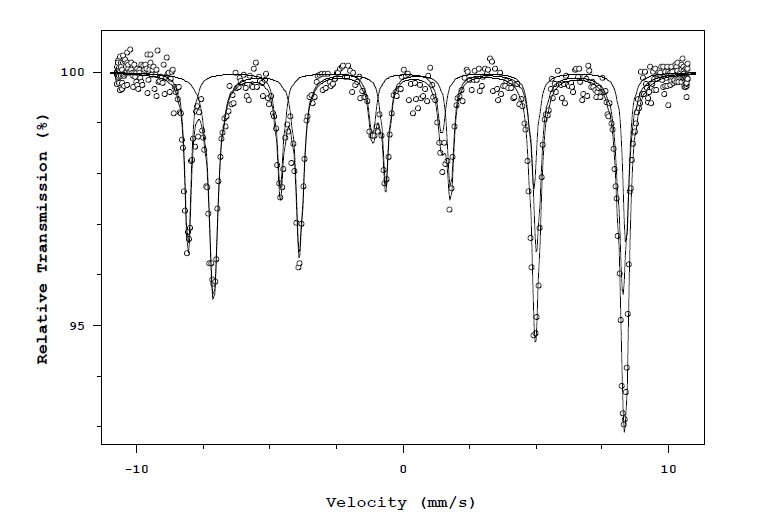
\includegraphics[scale=.5]{Bilder/Graph.png} 
	



\end{document}